\documentclass[11pt]{article}

\usepackage[hyphens]{url}

\usepackage[document]{ragged2e}

\usepackage{hyperref}
\hypersetup
{
    breaklinks = true,
    allcolors = black,
    linktoc = all
}

\usepackage{mathtools}
\usepackage{amssymb}
\usepackage{stmaryrd}
\usepackage{graphicx}

\usepackage{multicol}
\setlength{\columnseprule}{0.4pt}

\usepackage{listings}
\lstloadlanguages{Haskell}
\lstset
{
    basicstyle=\small\ttfamily,
    flexiblecolumns=false,
    basewidth={0.5em,0.45em},
    literate={+}{{$+$}}1 {/}{{$/$}}1 {*}{{$*$}}1 {=}{{$=$}}1
            {>}{{$>$}}1 {<}{{$<$}}1 {\\}{{$\lambda$}}1
            {\\\\}{{\char`\\\char`\\}}1
            {->}{{$\rightarrow$}}2 {>=}{{$\geq$}}2 {<-}{{$\leftarrow$}}2
            {<=}{{$\leq$}}2 {=>}{{$\Rightarrow$}}2 
            {\ .}{{$\circ$}}2 {\ .\ }{{$\circ$}}2
            {>>}{{>>}}2 {>>=}{{>>=}}2
            {|}{{$\mid$}}1 {\$}{\$}1         
}

\usepackage[english]{babel}
\usepackage[utf8]{inputenc}
\usepackage{fancyhdr}
\pagestyle{fancy}
\fancyhf{}
\rhead{James Burton}
\lhead{ID: 4251529}
\fancyfoot[C]{\thepage}

\usepackage{titling}
\title
{ 
    \vspace{10em}
    G53IDS - Final Report \\
    \hfill \break
    \large Embedded Domain Specific Language for \\
    Describing Recipes in Haskell
}

\setlength{\droptitle}{-10em}

\author{James Burton - 4251529 - psyjb6}

\begin{document}
\maketitle
\newpage

% Abstract and Acknowledgements
% 4 sentence abstract
% State the problem
% Why it's an interesting problem
% What my solution achieves
% What follows from my solution

\newpage

\tableofcontents
\newpage

\section{Introduction and Motivation}
\subsection{Overview}
Consider the following recipe to make a cup of tea:
\begin{tt}
\small
\begin{lstlisting}
    - Boil some water
    - Pour over a teabag
    - Wait for 5 minutes
    - Remove the teabag
    - Add milk (optional)
\end{lstlisting}
\end{tt}

This is a very simple but useful recipe that many people
will perform, in some cases, many times a day over their lives.
What we can realise by looking at this recipe is that it actually
consists of many smaller recipes, such as boiling water and
combining tea with milk, performed in a certain order. This
raises the question, to what extent does the order matter and
to what extent can we rearrange things in order to make the recipe
more efficient? No doubt you have done this, maybe subconsciously,
while cooking at home. Furthermore which steps can be done
concurrently in the event that multiple people are cooking e.g.
in a professional kitchen with a full brigade?

\medbreak

Perhaps closer to computer science, we could also ask, how could
we instruct a robot to do this? After doing some research on
robotic chefs it appears that not a huge number exist.
There is one home cooking robot \cite{robot} which uses motion
capture in order to learn recipes. In my opinion this is rather
restrictive. It presumes that the human performs the recipe in
the optimal manner and it would be very difficult to model
a brigade system in this way. In reality there is a limited set
of fundamental actions that one becomes able to perform when
learning to cook. Recipes can then be performed using a sequence
of these actions. Representing recipes like this would allow us
to take a robot programmed to perform each of the fundamental
actions and tell it how to cook literally anything. This is the
same principle as taking code written in a high level language
and compiling it down into a sequence of low level actions in
assembly language.

\medbreak

What is needed is a consistent way of representing recipes to
a computer such that they can be manipulated in various ways
for example scheduling, calculation of cost or even generating
suggestions on how to improve the recipe. My contributions
to solving this problem are the following:

\begin{itemize}
    \item I have provided a set of combinators as an EDSL in Haskell and show that
    they can be used to describe a wide variety of recipes (Section 2).

    \item I have defined a set of actions needed to actually execute a recipe (Section 3).

    \item I have defined what it means for two recipes to be equal.

    \item I have scheduled recipes defined in the EDSL using a representation
    of a kitchen environment. The schedule is optimised based on the tree-like
    structure of recipes in the EDSL.
\end{itemize}

\subsection{DSLs and Haskell}
Domain Specific Languages (DSLs) are programming languages that
are designed for use in a certain problem domain rather than
being general purpose. As such they trade range of expression
for clarity of expression. A frequently used example of a DSL
is the popular SQL used for accessing databases.

\medbreak

Embedded Domain Specific Languages (EDSLs) are DSLs that are embedded
within another language, such as Haskell. This allows for
fast development as you no longer need to write your parser
or compiler; programs written in your EDSL can just be interpretted
as programs written using the language in which it is embedded.
Secondly it allows programs written in your language to be
manipulated using the full power of the host language. Taking
an example from this project, if recipes were specified as a DSL
then in order to schedule them, one would have to either expand
the DSL to handle scheduling or write something in another language
to interpret the recipes so that they can be scheduled. In this
case the recipe EDSL is in Haskell and as such a scheduler can
just be written in Haskell as it would for any other purpose thus
saving both time and unecessary extra code.

\medbreak

Haskell is a very popular language for writing EDSLs, examples
range from pretty printing \cite{pretty} to financial contracts \cite{contracts}.
Reasons for this include that the type checker catches many mistakes
and that Haskell has very lightweight function application syntax
allowing us to omit symbols such as brackets in many cases \cite{snoyman}.

\subsection{Deep and Shallow Embedding}
When writing an EDSL one must choose between deep and shallow embedding.
Deep embedding means that the DSL's abstract syntax tree (AST) is
represented using an algebraic data type. On the other hand, shallow
embedding doesn't have an AST and the language constructs exist purely
as mappings to their semantics.

\medbreak

Both of these approaches have their advantages. Deep embedding
allows us to transform the representation before evaluating
it however, every time we want to add a new language construct
then we need to add it to the AST and as such our data type
can become quite large. Similarly, all functions manipulating
the AST must be changed to accomodate the new construct. Shallow
embedding avoids these issues as it doesn't have an AST however,
it does mean that we are limited to a specific semantic domain.

\medbreak

For the recipe DSL I have decided to borrow some features from
both. The fundamental actions which compose a recipe use a
deep embedding allowing us to evaluate the recipes in multiple
semantic domains for example cost or time. The functions
exposed to the user represent more of a shallow embedding
which makes the definition of recipes much more concise and
means that any new combinator can be added trivially as long
as it can be represented as some construction of the deeply
embedded actions.

\section{Combinators}
\subsection{Initial Definitions}

\subsection{Sequencing Problem}
\subsection{Conditionals}
\subsection{Transactions}
\subsection{Moving to a Tree of Actions}
\subsection{Final Definitions}
\subsection{Custom Combinators}

\section{Deriving Equality}
In this section I shall discuss what it means for two recipes
to be equal and how that has been used with QuickSpec \cite{quickspec, quickspec2}
in order to find algebraic properties held by recipes.

\subsection{Topological Sorting}
When considering what it means for two recipes to be equal one
might consider that they must have the same ingredients
and the same actions must be performed on those ingredients,
in the same order.

\medbreak

Our recipe tree already encodes the ingredients and the actions
performed on them, they are nodes in the tree. Ordering of
actions in our tree is captured by their level in the tree.
We can see that the actions we could choose to perform first
are the leaves of the tree. If we then remove a leaf and perform
that action then the actions we can perform next are the new
leaves of the tree. We can use this to generate a list of all
the different orders that the actions of a recipe can be performed
in while creating the same recipe. We want a way of generating
all combinations of nodes such that nodes higher in the tree
appear after their children in the list thus preserving the
order of our actions.

\medbreak

This is known as topological sorting. I have implemented a
function in Haskell below which, given a recipe, returns a list
of all topological sorts of that recipe.

\begin{lstlisting}
    topologicals :: Recipe -> [[Action]]
    topologicals (Node a []) = [[a]]
    topologicals t = concat
        [map (a:) (topologicals' l) | l@(Node a _) <- ls]
        where
            topologicals' l = topologicals $ removeFrom t l
            ls = leaves t
\end{lstlisting}

As an example, consider this alternate definition for our
cup of tea recipe. 

\begin{lstlisting}
    cupOfTea' :: Recipe
    cupOfTea' = optional $ combine "mix" 
        ( removeAfter (minutes 5)
        $ combine "mix" teabag
        $ heatTo 100 water ) milk
\end{lstlisting}

In this version we combine our tea with milk rather than combing milk with our tea.
Printing the trees for this recipe gives a different result from our original recipe.

\begin{figure}[h]
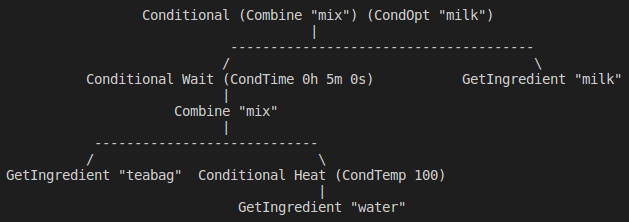
\includegraphics[width=\textwidth, keepaspectratio]{cupOfTea2.png}
\centering
\caption{Alternate cup of tea recipe printed as a tree.}
\end{figure}

In Haskell one must make their data type an instance of the \texttt{Eq} typeclass in
order to make use of the \texttt{==} operator. The equality instance for recipes is
defined as follows.

\begin{lstlisting}
    instance {-# OVERLAPPING #-} Eq Recipe where
        (==) r1 r2 = let xs = sort $ topologicals r1
                         ys = sort $ topologicals r2
                      in xs == ys
\end{lstlisting}

Because \texttt{Recipe = Tree Action} it naturally uses the equality instance for
\texttt{Tree} but we want to use our topological sorting. That's what the "overlapping"
annotation is for. As for the actual definition, we are simply taking the topological sorts
of each recipe, sorting them and then checking if those two lists are equal. If they are
then our recipes are equal. Using the above definition, the expression \texttt{cupOfTea == cupOfTea'}
evaluates to \texttt{True} showing that, as desired, our two recipes are equal.

\medbreak

As a side note \texttt{sort} requires an instance of \texttt{Ord} which means that values have some
natural order. This isn't defined for \texttt{Tree} by default and as such I have defined it as follows.

\begin{lstlisting}
    instance Eq a => Ord (Tree a) where
        compare t1 t2 = compare (length t1) (length t2)
\end{lstlisting}

This simply compares trees based on their length i.e.
their number of nodes.

\subsection{Quickspec}

\section{Scheduling Recipes}
\subsection{Modelling a Kitchen}
\subsection{Scheduling Method}
\subsubsection{Linear Programming}
\subsubsection{Bin Packing}
\subsubsection{Implementing a Scheduler}

\section{Recipe Properties}
\subsection{Folding Over Recipes}
\subsection{Time and Cost}
\subsection{Generating Recipes}
\subsection{Improving Recipes}

\section{Development Process}
\subsection{Project Management}

\section{Evaluation and Testing}
\subsection{Test Recipes}
\subsection{QuickCheck}

\section{Summary and Reflections}
\subsection{Project Management}
\subsection{Contributions}
\subsection{Future Work}
\subsection{Reflections}

\section{Related Work}
\subsection{Pretty Printing}
\subsection{Financial Contracts}
\subsection{Deep vs Shallow Embedding}
\subsection{Regions}
\newpage

    \begin{thebibliography}{8}

        \bibitem{robot}
        The Guardian. 2015. \textit{Future of food: how we cook}.
        \url{https://www.theguardian.com/technology/2015/sep/13/future-of-food-how-we-cook}
        Online. Accessed April 2, 2018.

        \bibitem{hudak}
        Paul Hudak. Domain Specific Languages. Department of Computer
        Science, Yale University, December 15, 1997.

        \bibitem{snoyman}
        Michael Snoynman. O'Reilly Webcast: Designing Domain Specific
        Languages with Haskell. January 4, 2013.
        \url{https://www.youtube.com/watch?v=8k_SU1t50M8}
        Online. Accessed April 2, 2018.

        \bibitem{contracts}
        Simon Peyton Jones, Microsoft Research, Cambridge.
        Jean-Marc Eber, LexiFi Technologies, Paris. Julian Seward,
        University of Glasgow. Composing contracts: an adventure in
        financial engineering. August 17, 2000.

        \bibitem{pretty}
        John Hughes. The Design of a Pretty-printing Library.
        Chalmers Teniska Hogskola, Goteborg, Sweden. 1995.

        \bibitem{embedding}
        Josef Svenningsson. Emil Axelsson. Combining Deep and Shallow
        Embedding of Domain-Specific Languages. Chalmers University
        of Technology. February 27, 2015.

        \bibitem{contracts-pp}
        Simon Peyton Jones, Microsoft Research, Cambridge.
        Jean-Marc Eber, LexiFi Technologies, Paris. Julian Seward,
        University of Glasgow. Composing contracts: an adventure in
        financial engineering (PowerPoint Slides). August 17, 2000.
        \url{https://www.microsoft.com/en-us/research/publication/composing-contracts-an-adventure-in-financial-engineering/}

        \bibitem{core}
        Simon Peyton Jones. Into the Core - Squeezing Haskell into
        Nine Constructors. September 14, 2016.
        \url{https://www.youtube.com/watch?v=uR_VzYxvbxg}
        Online. Accessed April 2, 2018.

        \bibitem{hutton-fold}
        Graham Hutton. Fold and Unfold for Program Semantics. Department of
        Computer Science, University of Nottingham. September 1998.

        \bibitem{quickspec}
        Koen Claessen, Chalmers University of Technology. Nicholas Smallbone,
        Chalmers University of Technology. John Hughes, Chalmers and Quviq AB.
        QuickSpec: Guessing Formal Specifications using Testing.
        September 28, 2013.

        \bibitem{quickspec2}
        Nicholas Smallbone. Moa Johansson. Koen Claessen. Maximilian Algehed.
        Chalmers University of Technology.
        Quick Specifications for the Busy Programmer. January 31, 2017.

    \end{thebibliography}   

    \newpage

    \appendix

\end{document}